\begin{frame}
	\frametitle{\problemtitle}
	\bigskip
	\bigskip
	\begin{block}{Problem}
		Given $n$ types of bricks $b_1,\dots,b_n$, can you build a wall of width $w$ where no two gaps appear above each other?
	\end{block}
	\bigskip
	\bigskip
	\bigskip
	\centering
	
\includegraphics[width=0.66\textwidth]{sample}
\end{frame}

\begin{frame}
	\frametitle{\problemtitle}
	\begin{block}{Subtask}
		Can at least one row be built?
	\end{block}
	\pause
	\begin{block}{Solution}
		This is known as the \emph{coin change problem} and can be solved like this:
		\begin{itemize}
			\item $\mathcal{O}(\frac{w^2}{64})$ with dp + bitsets
			\item $\mathcal{O}(w\log(w)^2)$ with fft \quad\textcolor{gray}{(faster is possible)}
			\pause
			\smallskip
			\item Bitsets are much faster
		\end{itemize}
	\end{block}

\end{frame}

\begin{frame}
	\frametitle{\problemtitle}
	\begin{columns}
		\begin{column}{0.4643\textwidth}
			\begin{block}{Case 1}
				\begin{itemize}
					\item $w\in\{b_1,\dots,b_n\}$
				\end{itemize}
				\vspace*{-0.5\baselineskip}
				\centering
				
\includegraphics[width=0.94\textwidth]{case1}
			\end{block}			
			\pause
			\begin{block}{Case 2}
				\begin{itemize}
					\item There is a row that uses two bricks $b_x$,$b_y$
					\pause
					\item WLOG:
					\begin{itemize}
						\item Let $b_x$ be the shortest
						\item Let $b_y$ be the second shortest
						\item there are as few $b_x$ as possible\\
						\textcolor{gray}{(still at least one)}
					\end{itemize}
				\end{itemize}
			\end{block}
		\end{column}
		\begin{column}{0.4643\textwidth}
			\pause
			\begin{block}{Case 2.1}
				\begin{itemize}
					\item Sum of $b_x$ can be replace by some $b_y$
				\end{itemize}
				\vspace*{-0.5\baselineskip}
				\centering
				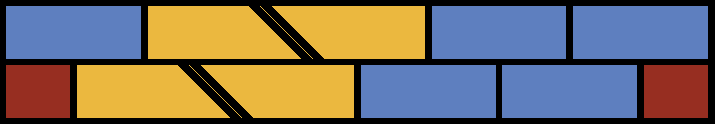
\includegraphics[width=0.94\textwidth]{case2.1}
			\end{block}
			\pause
			\begin{block}{Case 2.2}
				\begin{itemize}
					\item Else\strut
				\end{itemize}
				\vspace*{-0.5\baselineskip}
				\centering
				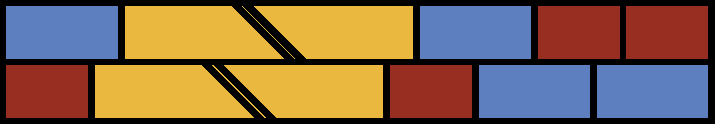
\includegraphics[width=0.94\textwidth]{case2.2}
			\end{block}
		\end{column}
	\end{columns}
\end{frame}

\begin{frame}
	\frametitle{\problemtitle}
	\begin{columns}
		\begin{column}{0.4643\textwidth}
			\begin{block}{Case 3}
				\begin{itemize}
					\item There are two bricks $b_x$,$b_y$ that divide $w$
					\pause
					\item Case 2 implies that $\mathit{lcm}(b_x,b_y)=w$
				\end{itemize}
				\vspace*{-0.5\baselineskip}
				\centering
				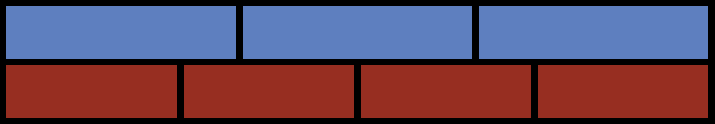
\includegraphics[width=0.94\textwidth]{case3}
			\end{block}	
		\end{column}
		\begin{column}{0.4643\textwidth}
			\pause
			\begin{block}{Case 4}
				\begin{itemize}
					\item Impossible
				\end{itemize}
			\end{block}
		\end{column}
	\end{columns}
	\begin{block}{Conclusion}
		The solution exists in two cases:
		\begin{itemize}
			\item Trivial: $w\in\{b_1,\dots,b_n\}$
			\item There exist two bricks that both can be part of a solution
		\end{itemize}
	\end{block}
	\pause % For some reason, this slide needs an extra \pause
	\solvestats
\end{frame}
